%&latex
%
\providecommand{\main}{../..}
\documentclass[../../main.tex]{subfiles}

\begin{document}

\subsection{Extinction time for a random walk} %TODO Move to previous section
Consider a particle moving on a $d=1$ integer lattice. At every position $m$, it may take a step \textit{to the right} ($m \to m+1$) or \textit{to the left} ($m \to m-1$) with equal rates $w$ (fig. \ref{fig:random_walk_mc}). However, when $m=0$ is reached, the particle stops moving \textit{forever}, i.e. $m=0$ is an \textbf{absorbing} state for the system.

\begin{figure}[H]
    \centering
    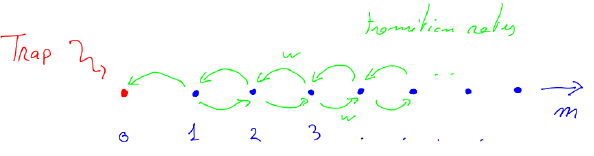
\includegraphics[width=0.8\textwidth]{random_walk_mc.png}
    \caption{Random walk on a $d=1$ integer lattice.}
    \label{fig:random_walk_mc}
\end{figure}

The Master Equation can be written as:
\begin{align}\label{eqn:random-walk-ME}
    \dot{\mathbb{P}}(m;t) &= w[\mathbb{P}(m-1;t) + \mathbb{P}(m+1;t) - 2 \mathbb{P}(m;t)] \qquad m \geq 2\\ \nonumber
    \dot{\mathbb{P}}(1;t) &= w[\mathbb{P}(2;t) - 2\mathbb{P}(1;t)]\\ \nonumber
    \dot{\mathbb{P}}(0,t) &= w \mathbb{P}(1;t)
\end{align}
In fact, every state $m \geq 2$ has exactly $2$ \textit{inward} transitions (with a \textit{positive} rate), and $2$ outward transitions (with a \textit{negative} rate). $m=1$ has only $1$ \textit{inward} and $2$ \textit{outward}, and $m=0$, being absorbing, has only \textit{inward} transitions (just the one from $m=1$).

\medskip

Since the particle never escapes the system, probability is conserved:
\begin{align}\label{eqn:random-walk-p-conv}
    \sum_{m=0}^{+\infty} \mathbb{P}(m,t) = 1 \qquad \forall t \geq 0
\end{align}
Indeed, if we assume that (\ref{eqn:random-walk-p-conv}) holds for $m=0$, then using (\ref{eqn:random-walk-ME}) we can prove it will hold for all $m > 0$.

\medskip

Note also that (\ref{eqn:random-walk-p-conv}) do not depend on $\mathbb{P}(0;t)$ when $m \geq 1$. 

\medskip

We can merge the $m \geq 2$ case with $m=1$ by defining:
\begin{align*}
    \hat{\mathbb{P}}(m;t) \equiv \begin{cases}
        \mathbb{P}(m;t) & m > 0\\
        0 & m = 0
    \end{cases}
\end{align*}
Then:
\begin{align}\label{eqn:random-walk-ME2}
    \dot{\hat{\mathbb{P}}}(m;t) = w [\hat{\mathbb{P}}(m-1;t) + \hat{\mathbb{P}}(m+1,t) - 2\hat{\mathbb{P}}(m;t)] \qquad m\geq 1
\end{align}
since when $m = 1$, the $m-1$ term vanishes.

\medskip

We can then use (\ref{eqn:random-walk-p-conv}) to determine the absorption probability $\mathbb{P}(0;t)$ from a solution of (\ref{eqn:random-walk-ME2}) as follows:
\begin{align}\label{eqn:random-walk-pzero}
    \mathbb{P}(0;t) = 1 - \sum_{m=1}^\infty \hat{\mathbb{P}}(m;t) 
\end{align}

Suppose the particle starts in $m_0$ at $t=0$, i.e. $\mathbb{P}(m,t=0) = \delta_{m,m_0}$. If $m_0 = 0$, the evolution is trivial: the particle will always remain in the absorbing state. Otherwise we have:
\begin{align*}
    \hat{\mathbb{P}}(m,t=0) = \delta_{m,m_0} \qquad m_0 \geq 1
\end{align*}

To solve (\ref{eqn:random-walk-ME2}), we first consider its extension to the \textit{whole} line $\mathbb{Z}$:
\begin{align}\label{eqn:random-walk-whole-line}
    \dot{\tilde{\mathbb{P}}}(m;t) = w[\tilde{\mathbb{P}}(m-1;t) + \tilde{\mathbb{P}}(m+1;t) - 2 \tilde{\mathbb{P}}(m;t)] \qquad m \in \mathbb{Z}
\end{align} 
The idea is that, on the whole line, we can use Fourier transforms to solve the differential equation.

To relate a solution of (\ref{eqn:random-walk-whole-line}) to one of (\ref{eqn:random-walk-ME2}) we use an argument of \textbf{symmetry}. By definition, we need $\hat{\mathbb{P}}(0;t) = 0$ - which is a condition that is automatically satisfied by \textit{odd} functions. 

So, let's take a solution $\tilde{\mathbb{P}}(m;t)$ of (\ref{eqn:random-walk-whole-line}) and make it \textit{odd}:
\begin{align}\label{eqn:odd-sol}
    \tilde{\mathbb{P}}_{\mathrm{odd}}(m;t) \equiv \tilde{\mathbb{P}}(m;t) - \tilde{\mathbb{P}}(-m;t)
\end{align} 
This function satisfies (\ref{eqn:random-walk-ME2}) for all $m \geq 1$:
\begin{align*}
    \dot{\tilde{\mathbb{P}}}_{\mathrm{odd}}(m;t) &= \dot{\tilde{\mathbb{P}}}(m;t) - \dot{\tilde{\mathbb{P}}}(-m;t) \underset{\mathclap{(\ref{eqn:random-walk-whole-line})}}{=}  w \Big[ \tilde{\mathbb{P}}(m+1;t) + \tilde{\mathbb{P}}(m-1,t) - 2 \tilde{\mathbb{P}}(m,t) +\\
    &\hspace{11em}\>\> - \tilde{\mathbb{P}}(-m-1;t) - \tilde{\mathbb{P}}(-m+1;t) + 2\tilde{\mathbb{P}}(-m;t) \Big] =\\
    &= w[\tilde{\mathbb{P}}_{\mathrm{odd}}(m+1;t) + \tilde{\mathbb{P}}_{\mathrm{odd}}(m-1;t) - 2 \tilde{\mathbb{P}}_{\mathrm{odd}}(m;t)]
\end{align*}
and also:
\begin{align*}
    \tilde{\mathbb{P}}_{\mathrm{odd}}(0;t) = \tilde{\mathbb{P}}(0;t) - \tilde{\mathbb{P}}(0;t) \equiv 0
\end{align*}
If we choose for $\tilde{\mathbb{P}}(m;t)$ the same initial condition $\delta_{m,m_0}$ we use for $\hat{\mathbb{P}}(m;t)$, then:
\begin{align*}
    \tilde{\mathbb{P}}_{\mathrm{odd}}(m;t=0) = \delta_{m,m_0} - \delta_{-m,m_0} \equiv \delta_{m,m_0} \quad \forall m \geq 1, m_0 \geq 1
\end{align*}
This means that given a solution of (\ref{eqn:random-walk-whole-line}) on the whole line, we can construct another solution $\tilde{\mathbb{P}}_{\mathrm{odd}}(m;t)$ according to (\ref{eqn:odd-sol}) that, when restricted to $m \geq 1$, satisfies the equation (\ref{eqn:random-walk-ME2}) we are interested to solve.

\medskip

Thus, all we need to solve is (\ref{eqn:random-walk-whole-line}) with $\tilde{\mathbb{P}}(m,0) = \delta_{m,m_0}$ with $m_0 > 0$ as initial condition, and $m \in \mathbb{Z}$. This can be done exactly in $d=1$ by using the Fourier series.

\medskip

For simplicity, we first take the continuum limit, and then solve. We start by constructing a pdf $\tilde{\mathbb{P}}(x,t)$ with $x \in \mathbb{R}$ as follows:
\begin{align*}
    \tilde{\mathbb{P}}(x,t) = \frac{1}{a} \tilde{\mathbb{P}}(m,t) \qquad x \in [ma,(m+1)a)
\end{align*} 
Graphically, $\tilde{\mathbb{P}}(m,t)$ is the area of the $m$-th \textit{bin}, which has a width of $a$, and so an height (probability density) of $\tilde{\mathbb{P}}(m,t) / a$. In the continuum limit $a \to 0^+$, $\tilde{\mathbb{P}}(x,t)$ becomes a \textit{smooth} function, that can be expanded. In particular:
\begin{align*}
    \tilde{\mathbb{P}}(m\pm 1, t) = \tilde{\mathbb{P}}(x\pm a, t) a = a \Big[\tilde{\mathbb{P}}(x,t) \pm a \tilde{\mathbb{P}}'(x,t) + \frac{a^2}{2} \tilde{\mathbb{P}}''(x,t) + \dots \Big]
\end{align*} 
Substituting in (\ref{eqn:random-walk-whole-line}) and ignoring $O(a^4)$ terms we get:
\begin{align*}
    \dot{\tilde{\mathbb{P}}}(x,t) = D \tilde{\mathbb{P}}''(x,t) \qquad \tilde{\mathbb{P}}(x,t=0) = \delta(x-x_0)
\end{align*}
where $D = w a^2$ is fixed in the continuum limit ($a \to 0$, $w \to \infty$), and $x_0 = m_0 a$.

\medskip

This is just the diffusion equation, in its most basic case. By Fourier transforming both sides, we can find the solution on the \textit{whole line}:
\begin{align*}
    \tilde{\mathbb{P}}(x,t) = \frac{1}{\sqrt{4 \pi D t}} \exp\left(-\frac{(x-x_0)^2}{4 D t} \right)
\end{align*}

To find the solution on the half line we use (\ref{eqn:odd-sol}):
\begin{align*}
    \hat{\mathbb{P}}(x,t) &\equiv \tilde{\mathbb{P}}_{\mathrm{odd}}(x,t) = \tilde{\mathbb{P}}(x,t) - \tilde{\mathbb{P}}(-x,t) =\\
    &=  \frac{1}{\sqrt{4 \pi D t}} \Big[ \exp\left(-\frac{(x-x_0)^2}{4 D t} \right) - \exp\left(-\frac{(x+x_0)^2}{4 D t} \right) \Big]
\end{align*}

We can then verify the required properties:
\begin{enumerate}
    \item \textbf{Initial condition}:
    \begin{align*}
        \hat{\mathbb{P}}(x,0^+) = \delta(x-x_0) - \delta(x+x_0) = \delta(x-x_0) \qquad \forall x,x_0 > 0
    \end{align*} 
    \item \textbf{Boundary condition}:
    \begin{align*}
        \hat{\mathbb{P}}(0,t) \equiv 0 \qquad \forall t
    \end{align*} 
    \item \textbf{Probability conservation}:
    \begin{align*}
        \int_0^\infty \hat{\mathbb{P}}(x,t) \dd{x} &= \erf \left(\frac{x_0}{\sqrt{4 D t}} \right) < 1 \qquad \forall t\\
        \erf(x) &\equiv \frac{2}{\sqrt{\pi}} \int_0^x e^{-y^2}\dd{y}
    \end{align*} 
    So, apparently, probability \textbf{is not} conserved. However, recall that the original probability conservation (\ref{eqn:random-walk-p-conv}) involves $\mathbb{P}(m,t)$, not $\hat{\mathbb{P}}(m,t)$. The integral we just computed is rather the \textbf{survival probability}, i.e. the probability that the particle is not absorbed in $m=0$ at time $t$.
    
    This can be shown by taking the continuum limit of (\ref{eqn:random-walk-pzero}):
    \begin{align*}
        \mathbb{P}(0,t) = 1 - \sum_{m \geq 1} \hat{\mathbb{P}}(m,t)  \xrightarrow[a \to 0]{}  1 - \int_0^\infty \hat{\mathbb{P}}(x,t)\dd{x} \equiv 1 - \mathcal{P}_>(t|m_0)
    \end{align*} 
    where $\mathcal{P}_>(t|m_0)$ is the survival probability at time $t$ for a particle withi initial position $m_0$. Thus:
    \begin{align}\label{eqn:random-walk-psurv}
        \mathcal{P}_>(t|x_0) = \erf\left(\frac{x_0}{\sqrt{4 D t}} \right)
    \end{align}

    Recall that, for a random walk, the mean square displacement after time $t$ is:
    \begin{align*}
        \xi^2(t) \equiv \langle x^2 \rangle_t = 2Dt
    \end{align*}
    This defines a characteristic \textit{length scale} for the random walk, and so we can rewrite (\ref{eqn:random-walk-psurv}) as a scaling law depending only on the \textit{dimensionless} variable $x_0/\xi(t)$:
    \begin{align*}
        \mathcal{P}_{>}(t|x_0) \equiv f\left(\frac{x_0}{\xi(t)} \right) \sim \begin{cases}
            t^{-1/2} & t \gg \frac{x_0^2}{2 D} \equiv \tau_c\\
            1 & t \ll \frac{x_0^2}{2D} \equiv \tau_c  
        \end{cases}
    \end{align*} 
    where we have used the MacLaurin expansion of the $\erf$ function:
    \begin{align*}
        \erf(x) \underset{x\approx 0}{=}  \frac{2}{\sqrt{\pi}} \left(x - \frac{x^3}{3} + O(x^5) \right) 
    \end{align*}
    Then using (\ref{eqn:lifetime-derivative}, pag. \pageref{eqn:lifetime-derivative}) we obtain the lifetime distribution (i.e. the distribution of the time interval required to reach $m=0$ for the first time for a particle starting in $x_0$):
    \begin{align*}
        \mathcal{P}(t|x_0) &= - \pdv{t} \mathcal{P}_> (t|x_0) = -\pdv{t} \frac{2}{\sqrt{\pi}} \int_0^{\frac{x_0}{\sqrt{4 D t}} } e^{-x^2} \dd{x} =\\
        &= \frac{1}{t} F\left(\frac{x_0}{\xi(t)} \right) \sim t^{-3/2} \qquad t \gg \tau_c\\
        F(x) &= \frac{1}{\sqrt{4 \pi}} x \exp\left(-\frac{x^2}{2} \right)
    \end{align*}
%TODO Compare the exponents above with the case of the birth-death process
\end{enumerate}

\begin{exo}[Lifetime distribution with Fisher Log-Series]
    \begin{enumerate}[label=(\alph*)]
        \item Use the exact result (\ref{eqn:lifetime-pdf}, pag. \pageref{eqn:lifetime-pdf}) to determine the lifetime distribution of species in a system whose stationary distribution is the Fisher Log-Series, i.e. the probability to find a species with population $n_0$ is given by:
        \begin{align*}
            \mathbb{P}_{n_0}^{\mathrm{stat} } = \frac{\alpha}{n_0} \left(\frac{b}{d} \right)^{n_0} \qquad b < 1, \> d-b = \delta = \frac{1}{\tau_c} 
        \end{align*}
        with $\alpha^{-1} = |\ln(1- b/d)|$.
        \item Use the result from (a) to determine if there is scaling in the regime $\delta \to 0^+$ and $t \to +\infty$ with $\delta \cdot t$ fixed. If so, determine the exponents in the $t \ll \tau_c$, and draw a plot of the relevant behaviour.
    \end{enumerate}    
\end{exo}

\section{The Voter Model}\label{sec:voter-model}
\lesson{33}{25/05/20}

The \textbf{voter model} was originally created in 1975 by Richard A. Holley and Thomas M. Liggett to describe the evolution of people's opinions on polytical parties as consequence of peer pressure.

\medskip

In its most basic form,\marginpar{Basic voter model} each \q{voter} may choose between two possibilities $0$ or $1$, and their beliefs are influenced by their neighbours - meaning that someone voting $1$ that happens to be amongst a group where everyone votes $0$ is likely to change opinion after some time, simply because they hear a lot about $0$.

\medskip

The voter model can be generalized to describe a ecosystem\marginpar{Voter model for ecosystems} with $S$ \textbf{species} (the parties), where each \textbf{node} (person) belongs to one of them, and sits at a position in a $d$ dimensional lattice. Then a \q{person changing ideas} corresponds to a individual of a certain species \textit{dying} and being replaced by a new organism of the neighbouring species - or eventually with an individual of an entirely new species.  

\medskip

To simplify things,\marginpar{Spin-like \textbf{States}} let's focus on only one specific species $A$. Then we define the state $\sigma_x$ of node $x$ as a spin-like variable:
\begin{align*}
    \sigma_x = \begin{cases}
        +1 & \text{if node $x$ is occupied by species $A$}\\
        -1 & \text{otherwise}
    \end{cases}
\end{align*}

At each timestep $n$ \marginpar{\textbf{Dynamics}} a random node $x$ is selected, and the value of $\sigma_x$ is replaced by $\sigma_y$, where $y$ is a randomly chosen \textbf{nearest neighbour} (n.n.) of $x$ \hbox{($y \in \langle x,y \rangle$)}. 

\medskip

Let $w_x(\bm{\sigma})$ be the probability per unit time (i.e. the rate) that spin $\sigma_x$ in state $\bm{\sigma}$ is flipped, i.e. that the transition $\sigma_x \to -\sigma_x$ occurs (leaving all other spins unchanged). 

If all the neighbours of $x$ are equal to $-\sigma_x$, then the transition rate is maximum, and we fix it as $w_x(\bm{\sigma}) \overset{!}{=} 2w$, where $w$ is proportional to the system's \q{reaction speed}, i.e. the reciprocal of its characteristic time $\tau_c$. Conversely, if all neighbours of $x$ are in the same state $\sigma_x$, then no flip will ever occur: $w_x(\bm{\sigma}) = 0$. 

For all the in-between cases, we use a linear interpolation, making the spin-flip rate proportional to the fraction of neighbours of $x$ that \textit{disagree} with $\sigma_x$. Since each node in a $d$-dimensional cubic lattice has $2d$ neighbours, we arrive to the following expression for $w_x(\bm{\sigma})$:
\begin{align}\label{eqn:spin-change1}
    w_x(\bm{\sigma}) = \left[1- \frac{1}{2d}(n_{\sigma_x} - n_{-\sigma_x}) \right] w = \frac{n_{-\sigma_x}}{d} w 
\end{align}
where $n_{\pm \sigma_x}$ is the number of n.n. of $x$ with state $\pm \sigma_x$.

Note that if $\sigma_y = \sigma_x$, then $\sigma_y \sigma_x = +1$, and otherwise we have $\sigma_y \sigma_x = -1$. So:
\begin{align*}
    n_{\pm \sigma_x} = \pm \sum_{\mathclap{y \in \langle x,y \rangle}} \sigma_x \sigma_y
\end{align*}
And substituting back in (\ref{eqn:spin-change1}) leads to:
\begin{align}\label{eqn:spin-change2}
    w_x(\bm{\sigma}) = \left[1 - \frac{1}{2d} \sigma_x \sum_{\mathclap{y \in \langle x,y \rangle}} \sigma_y \right] \cdot w
\end{align}
Then, similarly to what we did in sec. \ref{sec:dynamics-ising}, the transition rate from state $\bm{\sigma'}$ to any other state $\bm{\sigma}$ can be written as the sum over the necessary spin-flip transitions:
\begin{align*}
    W(\bm{\sigma}|\bm{\sigma'}) = \sum_x w_x(\sigma) \delta_{\sigma_x, -\sigma_x'}\Big[ \prod_{z \neq x} \delta_{\sigma_z', \sigma_z} \Big]
\end{align*}

\begin{figure}[H]
    \centering
    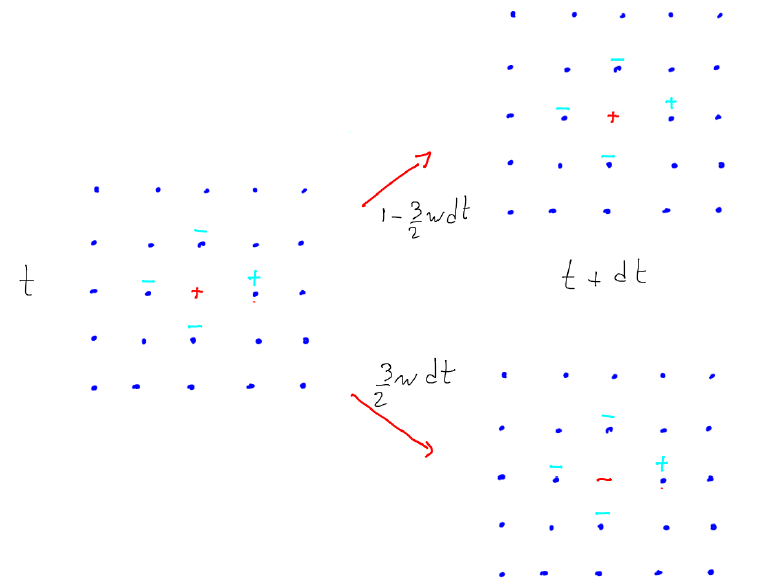
\includegraphics[width=0.8\textwidth]{spin-flips.png}
    \caption{Example of spin-flip transitions on a $d=2$ lattice. The red $\textcolor{Red}{+1}$ spin has $1$ neighbour \textit{agreeing} with it ($n_{+1} = 1$) and $3$ that \textit{disagree} with it ($n_{-1} = 3$). The maximum possible flip rate is $2w$, but since only $3/4$ of neighbours disagree, the final rate will be $3w/2$, leading to a transition \textbf{probability} of $3w \dd{t}/2$. Conversely, the transition probabilities with \textit{no spin-flip} will be $1-3w\dd{t}/2$.}
    \label{fig:spin-flips}
\end{figure}

Let $\bm{\sigma}$ be a spin configuration, and denote with $\bm{\sigma^{(x)}}$ the configuration resulting from flipping \textit{only} spin $x$ of $\bm{\sigma}$, i.e. such that:
\begin{align*}
    \sigma_x^{(x)} = -\sigma_x; \qquad \sigma_y^{(x)} = \sigma_y \quad \forall y \neq x
\end{align*} 
We can then write the system's Master Equation:\marginpar{\vspace{2em}Master Equation}
\begin{align}\label{eqn:voting-ME}
    \dot{P}(\bm{\sigma};t) = \sum_x [\underbrace{w_x(\bm{\sigma^{(x)}}) \mathbb{P}(\bm{\sigma^{(x)}}; t)}_{\text{\q{Inward} flux}}  - \underbrace{w_x(\bm{\sigma}) \mathbb{P}(\bm{\sigma}; t)}_{\text{\q{Outward} flux}} ]
\end{align}

% Two key questions:
% \begin{enumerate}
%     \item What is the probability that a certain species will persist forever?
%     \item In which conditions can many species coexist?
% \end{enumerate}

\subsection{Correlation functions}
In order to get some insight on the dynamics, we compute the evolution of the $1$ and $2$-point correlation functions.

\subsubsection{1-point correlation}

First, consider the following change of variables, from \textit{spin}-like ($\pm 1$) to \textit{binary} ($\{0,1\}$):
\begin{align}\label{eqn:presence-indicator}
    \frac{1+\sigma_z}{2} = \begin{cases}
        1 & \text{if the chosen species is occupying node $z$}\\
        0 & \text{otherwise}
    \end{cases} 
\end{align}  
The probability that a given species is present at $x$ at time $t$ is given by averaging the indicator \textit{binary} variable of \q{presence} over all nodes:
\begin{align*}
    \langle \frac{1+ \sigma_z}{2}  \rangle_t = \frac{1+\langle \sigma_z \rangle_t}{2} 
\end{align*}


\end{document}
